\let\cleardoublepage\clearpage
\chapter{Химическая технология}
\ID{МРНТИ 61.74.31}{}

\begin{articleheader}
\sectionwithauthors{Ж.Б. Ильмалиев, Қ.А. Куртибай, Ә. Қаппасулы, Е.Е. Жатқанбаев, Э.Б. Жунусова, Г.Б. Ильмалиева, А.К. Жумабекова}{СОЗДАНИЕ И ИЗГОТОВЛЕНИЕ КОМПОЗИТОВ НА ОСНОВЕ ОТХОДОВ ДРЕВЕСИНЫ}

{\bfseries
\textsuperscript{1}Ж.Б. Ильмалиев,
\textsuperscript{2}Қ.А. Куртибай,
\textsuperscript{2}Ә. Қаппасулы\textsuperscript{\envelope },
\textsuperscript{3}Е.Е. Жатқанбаев,
\textsuperscript{3}Э.Б. Жунусова,
\textsuperscript{1}Г.Б. Ильмалиева,
\textsuperscript{3}А.К. Жумабекова,
}
\end{articleheader}

\begin{affiliation}
\textsuperscript{1} ТОО «URBAN GROUP», Алматы, Казахстан,

\textsuperscript{2} ТОО «Научно-производственный центр экологической и промышленной биотехнологии», Астана, Казахстан,

\textsuperscript{3} Казахский университет технологии и бизнеса имени К. Кулажанова, Астана, Казахстан,

\raggedright \textsuperscript{\envelope } Корреспондент-автор: kappasuly@mail.ru
\end{affiliation}

Статья посвящена разработке и производству арболита - легкого
крупнопористого бетона на основе органического древесного наполнителя и
минерального вяжущего. В статье рассмотрены этапы подготовки
производства, технологический процесс производства и особенности
применения арболита в строительстве. В статье акцентируется внимание на
преимуществах арболита, таких как высокая тепло- и звукоизоляция,
огнестойкость, биостойкость и прочность, что делает его перспективным
шагом для малоэтажного строительства и использования в зонах с высокой
пожарной опасностью.

Одним из важных аспектов исследования является использование золы
теплоэлектростанций (ТЭЦ) в качестве минеральной добавки, что позволяет
снизить себестоимость производства и решить проблему утилизации
промышленных отходов. Экспериментальные данные о том, что арболитовые
блоки, изготовленные с добавлением зол, обеспечивают получение
физико-механических характеристик, соответствующих строи.

Исследования также затрагивают вопросы безопасности производства,
включая переработку древесных отходов и использование нетоксичных
компонентов. Технология производства арболита, описанная в статье,
проста и эффективна, что делает ее перспективной для широких разработок
в строительной отрасли Казахстана. Результаты работы показывают
актуальность использования арболита в условиях изменчивого климата и
высоких требований к теплоизоляции.

{\bfseries Ключевые слова:} арболит, древесные отходы, минеральные вяжущие,
теплоизоляционные материалы, зола теплоэлектростанций, экологически
чистые строительные материалы, огнестойки.

\begin{articleheader}
{\bfseries АҒАШ ҚАЛДЫҚТАРЫ НЕГІЗІНДЕ КОМПОЗИТТЕРДІ ЖАСАУ ЖӘНЕ ӨНДІРУ}

{\bfseries
\textsuperscript{1}Ж.Б. Ильмалиев,
\textsuperscript{2}Қ.А. Куртибай,
\textsuperscript{2}Ә. Қаппасұлы\textsuperscript{\envelope },
\textsuperscript{3}Е.Е. Жатқанбаев,
\textsuperscript{3}Э.Б. Жунусова,
\textsuperscript{1}Г.Б. Ильмалиева,
\textsuperscript{3}А.К. Жумабекова,
}
\end{articleheader}

\begin{affiliation}
\textsuperscript{1}«URBAN GROUP» ЖШС, Астана, Қазақстан,

\textsuperscript{2}«Экологиялық және өнеркәсіптік биотехнология ғылыми-өндірістік орталығы» ЖШС, Астана, Қазақстан,

\textsuperscript{3}Қ. Қулажанов атындағы Қазақ технология және бизнес университеті, Астана, Қазақстан,

e-mail: kappasuly@mail.ru
\end{affiliation}

Мақала ағаш органикалық толтырғышы мен минералды байланыстырғыш
негізінде жасалған жеңіл ірі кеуекті бетон - арболитті әзірлеу мен
өндіруге арналған. Онда өндірісті дайындау кезеңдері, өндіріс
технологиялық үдерісі және арболиттің құрылыста қолданылу ерекшеліктері
қарастырылған. Мақалада арболиттің жылу және дыбыс оқшаулау, отқа
төзімділік, биологиялық тұрақтылық және беріктік сияқты артықшылықтарына
назар аударылады. Бұл оны аз қабатты құрылыс пен өрт қаупі жоғары
аймақтарда қолдануға болашағы зор етеді.

Зерттеудің маңызды аспектілерінің бірі ретінде жылу электр
станцияларының (ЖЭС) күлін минералды қоспа ретінде қолдану ұсынылған.
Бұл өндіріс шығындарын азайтуға және өндірістік қалдықтарды кәдеге
жарату мәселесін шешуге мүмкіндік береді. Эксперименттік мәліметтер
арболит блоктарының құрамына күл қосылған жағдайда,
физикалық-механикалық қасиеттерінің құрылыс талаптарына сәйкес келетінін
көрсетеді.

Зерттеулер өндірістің қауіпсіздігі, соның ішінде ағаш қалдықтарын қайта
өңдеу және улы емес компоненттерді пайдалану мәселелерін де қамтиды.
Мақалада сипатталған арболит өндірісі технологиясы қарапайым әрі тиімді,
бұл оны Қазақстанның құрылыс саласында кеңінен қолдануға мүмкіндік
береді. Зерттеу нәтижелері арболиттің құбылмалы климат жағдайында және
жылу оқшаулауға жоғары талаптар қойылатын жерлерде қолданылуының
өзектілігін көрсетеді.

{\bfseries Түйін сөздер}: арболит, ағаш қалдықтар, минералды
байланыстырғыштар, жылу оқшаулау материалдары, ЖЭС күлі, экологиялық
таза құрылыс материалдары, отқа төзімділік.

\begin{articleheader}
{\bfseries DEVELOPMENT AND PRODUCTION OF COMPOSITES BASED ON WOOD WASTE}

{\bfseries
\textsuperscript{1}Zh.B. Ilmaliev,
\textsuperscript{2}K.A. Kurtybay,
\textsuperscript{2}A. Kappasuly\textsuperscript{\envelope },
\textsuperscript{3}Ye.E. Zhatkanbayev,
\textsuperscript{3}E.B. Zhunusova,
\textsuperscript{1}G.B. Ilmalieva,
\textsuperscript{3}A.K. Zhumabekova
}
\end{articleheader}

\begin{affiliation}
\textsuperscript{1}«URBAN GROUP» LLP ,Almaty, Kazakhstan,

\textsuperscript{2} LLP "Scientific and Production Center for Environmental and Industrial Biotechnology," Astana, Kazakhstan

\textsuperscript{3} K. Kulazhanov Kazakh University of Technology and Business, Astana, Kazakhstan

e-mail: kappasuly@mail.ru
\end{affiliation}

This article is dedicated to the development and production of
arbolite - a lightweight, large-porous concrete based on an organic wood
filler and mineral binder. It discusses the production preparation
stages, technological process, and features of using arbolite in
construction. The article emphasizes the advantages of arbolite, such as
high thermal and sound insulation, fire resistance, biological
stability, and strength, making it a promising material for low-rise
construction and use in areas with high fire risk.

One of the key aspects of the study is the utilization of thermal power
plant (TPP) ash as a mineral additive, which reduces production costs
and addresses the problem of industrial waste disposal. \\Experimental
data demonstrate that arbolite blocks produced with ash additives
achieve physical and mechanical characteristics that meet construction
standards.

The research also addresses production safety issues, including the
recycling of wood waste and the use of non-toxic components. The
arbolite production technology described in the article is simple and
efficient, making it a promising option for widespread adoption in
Kazakhstan's construction industry. The study results highlight the
relevance of using arbolite in conditions of variable climates and high
thermal insulation requirements.

{\bfseries Keywords}: arbolite, wood waste, mineral binders, thermal
insulation materials, thermal power plant ash, environmentally friendly
construction materials, fire resistance.

\begin{multicols}{2}
{\bfseries Введение.} К древесным композиционным материалам относят
матрицы, наполненные древесиной в различных ее видах. Для производства
подобных композиционных материалов - арболита, фибролита, стружкобетона,
скопобетона, опило-бетона, цементно-стружечных плит, королита,
ксилолита, применяются различные целлюлозосодержащие заполнители
растительного происхождения и в качестве минерального связующего
используются портландцемент или шлакощелочное вяжущие компоненты.

Древесно-цементные композиты обычно представляют собой нити, частицы или
волокна древесины, смешанные вместе с портланд- или шлакоцементом в
качестве минерального связующего и в зависимости от плотности можно
разделить на две группы: легкие, имеющие плотность менее 1200
кг/м\textsuperscript{3}, и тяжелые со средней плотностью более 1200
кг/м\textsuperscript{3} {[}1{]}. К легким можно отнести гипсостружечные
и гипсоволокнистые плиты, фибролит, арболит, королит, гипсоопилочные
блоки, ДВП, ДСП. Нами исследованы композиты, типа арболит, которые
обладают преимуществами цемента, это огнестойкость, устойчивость к
биодиструкции, высокая степень звукоизоляции, при легкости обработки,
высокой плотности при относительно легком весе. Производство
древесно-цементных композитов может быть перспективным способом
утилизации древесных отходов. Арболит, может быть использован, как для
внутренних, так и для наружных работ. Он легче бетона, имеет высокую
прочность на растяжение, повышенную трещиностойкость, достаточную
сопротивляемость ударным нагрузкам. Минеральные вяжущие придают
прочность, биостойкость, огнестойкость, морозостойкость, что расширяет
области применения как в сборных конструкциях, в элементах отделки и
звукоизоляции, малоэтажном строительстве и в производственных зданиях,
при отделке в качестве перегородок зданий различной этажности.

Изготавливаемый композиционный материал арболит, это крупнопористый
легкий бетон на основе органического наполнителя и минерального вяжущего
цемента. За счет органического, в данном случае древесного, наполнителя
снижается плотность, коэффициент теплопроводности. Повышается
звукоизоляционные свойства и обрабатываемость материала. За счет
минеральной, цементной части, изделиям придается прочность,
огнестойкость, морозостойкость и биостойкость и арболиты намного лучше
подходят для использования в местах с высокой степенью возгорания. В
зависимости от потребности рынка арболит может формироваться разной
плотности, по пределу прочности при сжатии 5, 10, 15
кг/см\textsuperscript{2} для теплоизоляции и 25, 35, 50
кг/см\textsuperscript{2} для конструкций. Так же композит производится в
форме панелей, кирпичей и плиток. При их производстве не выделяется
токсичных отходов, использование золы ТЭЦ в качестве минерального
связующего и древесных отходов в качестве наполнителя, что можно считать
утилизацией, позволяет создать экологичное производство строительных
товаров широкой области применения. Выше сказанное в свете решения
проблем с утилизацией отходов деревообрабатывающей промышленности и
энергетики, а также экологичного производства строительных материалов
является актуальной задачей {[}2-3{]}.

Результатом исследований и разработки технологии является производство
востребованной продукции - легких и прочных строительных блоков с
высокими физико-механическими и эксплуатационными свойствами. Снижение
трудоемкости при монтаже стеновых блоков, панелей, перекрытий, а так же
отделке поверхностей каркасов стен и фасадных работах, высокая
огнестойкость материала дает возможность широкого применения в
малоэтажном строительстве, а так же возведении зданий и сооружений с
повышенными требованию по теплорегуляции и звукоизоляции, а также
использование при реставрации и модернизации жилого и производственного
фондов в процессе производства вторичного сырья, при растущей
потребности в качественном и экологичном строительном материале,
производство арболита является актуальной задачей.

Качественный, недорогой и экологичный цементный композит высокой
прочности, может быть использован в строительстве и отделочных работах в
районах Казахстана с изменчивым климатом, различными погодными условиями
и температурными режимами.

Сырьевые ресурсы, надлежащая опытно - экспериментальная база и
отработанная технология позволяет получать композитные материалы
стабильно высокого качества, востребованные на рынке строительных
материалов РК.

Различные характеристики исходного сырья, условия производства и
хранения имеют значительное влияние на получаемые материалы. Влияние
добавок, как к примеру, внесение в цементное тесто двуокиси углерода,
позволяют производить древесно-цементные композиты в гораздо более
короткие сроки {[}4{]}. Добавки кремнеземной или изоцианатной смолы,
извести гидротатной, жидкого стекла также продемонстрировали улучшение
свойств продукта. Так же хлорид и нитрат кальция, нитрит-нитрат-хлорид
кальция, сернокислый глинозем, хлорид кальция плюс оксид кальция
ускоряют процесс твердения цемента. Использование древесных составляющих
вносит в процесс получения композита определенные сложности, это связано
со сложностью стандартизации природных материалов, древесины и
лигноцеллюлозы по компонентам, и степени несовместимости растительной
дисперсии с цементом. Испытание материалов, определение методов
производства и изменение технологических режимов, выполняется для
каждого вида растительного сырья. В литературных источниках имеются
данные показателях степени несовместимости, основанные на тепловых
характеристиках процесса схватывания и физических свойствах композитов,
степени гидратации портландцемента. Проблема химической совместимости
дерева и цемента иногда приводит к задержке или полному отсутствию
схватывания. Для увеличения адгезии может применяться разбавленный
щелочной раствор, для ускорения отверждения цемента, вводят добавки
хлоридов металлов олова, железа, алюминия, магния или кальция {[}5-8{]}.

Одно из современных направлений, это разработка и производство
композитных строительных материалов. Арболит, древесно --цементный
композит во многом отвечает данным требованиям. Этот композит можно
назвать целлюлозосодержащим материалом на основе цемента. Для получения
качественного материала. Отвечающего заданным характеристикам,
необходимо проводить исследования всех компонентов, условий и
технических режимов. В производстве строительных композитов широко
применяются растительные и древесные отходы. Производства, включающие
применение древесины, сопровождаются образованием большого количества
отходов, которые можно рентабельно использовать в производствах
стройматериалов. Древесина легко обрабатывается, обладает достаточно
высокой прочностью, имеет высокий коэффициент конструктивного качества,
малой коэффициент теплопроводности. Из недостатков, высокая
гигроскопичность, влагоемкость, горючесть и загниваемость. Так же
свойствам, осложняющих производство можно отнести наличие различных
структурных включений, сучков, трещин, разнослойности, а также усушку и
набухание. Обработка древесины позволяет значительно улучшить качество
древесины, т.е. частично устранить присущие ей недостатки и полностью
устранить отходы при ее переработке. Изменение свойств и характеристик
древесины влияет на изменение других физико-механических свойств
получаемых материалов, для стандартизации технологии важна
характеристика влажности, отслеживаемая в продолжении всего
технологического цикла, поэтому все результаты приводятся к условной 15
\% влажности. Испытанию древесины в лабораториях всегда предшествует
определение влажности образцов. При производстве арболитов так же важна
удельная поверхность частиц древесного наполнителя и структура
древесины. Для производства арболита применяют различные органические
заполнители, целлюлозосодержащий растительный продукт, свойства
которого, влияет на процессы структурообразования,
структурно-механические и теплотехнические свойства материала {[}9{]}.

Древесина имеет сложный состав и некоторые компоненты оказывают влияние
на свойства цементов. Отрицательное влияние на цемент оказывают
вещества: фенолы, полисахара, дубильные вещества, кислоты, хиноны.
Углеводы и дубильные вещества, входящие в состав древесины, являются
поверхностно-активными гидрофилизирующими веществами и препятствуют
сцеплению частичек древесного наполнителя с цементом. Для повышения
качества древесно-цементных композиционных материалов, содержащиеся в
древесине водорастворимые вещества, «Цементные яды», обезвреживаются
минерализацией, обработкой, пропиткой растворами хлорида кальция,
сернокислого глинозема, растворимым стеклом. Строение, достаточно хорошо
видимое невооруженным глазом или при слабом увеличении, называется
макроструктурой, а видимое при сильном увеличении в микроскоп
-микроструктурой. Макроструктура древесины. Исследованием макроструктуры
определяется зрелая древесина, все древесные породы подразделяют на я
дровые, имеющие ядро и заболонь, заболонные, имеющие только заболонную
древесину, и спело древесные, имеющие заболонь и спелую древесину
{[}10{]}. Для технологии предпочтительно использовать летнюю, а не
весеннюю древесину. Относительно пород древесины, лучшая щепа получается
из хвойных, сосны и ели, хорошие показатели и у лиственницы, осины,
бука, березы, тополя. Размеры устанавливаются опытным путем, максимально
длиной до 40мм, и оптимальная длина 25 мм при ширине 10 мм. По
содержанию коры до 10\%, мелкая фракция, и крупные включения
отсортировываются, не желательно примеси плесени и гнили. Из такого
сырья получаются самые прочные арболитовые блоки. Испытание древесины.
Исследуются характеристики сырья, которые могу повлиять на
технологический процесс. Влажность является важным показателем. По
степени влажности сырье древесины классифицируют, как древесину
свежесрубленную, влажность 35 \% и выше; воздушно-сухую влажность 15-20
\%; комнатно-сухую влажность 8-13 \%, мокрую, с большой влажность до 100
\% и более {[}10{]}.

{\bfseries Материалы и методы.} Состояние равновесной влажности в древесине
достигается при нахождении постоянных температура - влажностных условиях
длительное время. Зависит от упругости паров воды окружающего воздуха и
упругости паров воды на поверхности древесины. Строятся графики
зависимости и определяются заданные характеристики. Влажность и
температура воздуха определяется по психрометрическим таблицам с помощью
лабораторного психрометра. Для достижения равновесной влажности,
древесина должна находится на воздухе с постоянными относительной
влажностью и температурой, долгое время, при равности упругости паров
окружающего воздуха, а упругости паров поверхности древесины,
достигается влажность, называемая равновесной. Часто постоянная
влажность и температура, при которой хранится древесина недостижима, при
уличном складировании, для определения влажности древесины, находящейся
в условиях с различной температурой и влажностью окружающего воздуха,
используют графическую зависимость влажности от температуры, при
построении откладывают по ординате влажность воздуха, по абсциссе -
температуру воздуха, влажность древесины определяют по графикам, имеющим
вид наклонных линий. Графики, построенные по данной зависимости,
позволяют определить влажность с точностью до 0,75 \%. Есть метод
прямого определения, параметры рассчитываются по формуле (1).

\begin{equation}
W = \frac{m_{1} - m_{2}}{m_{2} - m}\  \times 100
\end{equation}

где,

m -- масса бюксы, г;

m1 - масса влажного образца с бюксой, г;

m2 - масса сухого образца с бюксой, г;

Определение усушки древесины.

Расчет влажности при прямом измерении. При необходимости более точного
определения параметров, влажность древесины определяется взвешивание
прямым путем. Древесина высушивается в сушильном шкафу,

разница между взвешиванием определяется экспериментально. Эксперимент
проводят в бюксе, в предварительно взвешенную бюксу помещают проба
древесины, снова взвешивается, затем происходит сушка с пробы в
сушильном шкафе. Пробу сушит не закрывая, эксперимент проводят до
постоянной массы. Значит древесина высушилась. Взвешивается с точностью
до 0,001 г. Температура в сушильном шкафе выдерживается 100˚C. Бюкса с
образцом взвешивается после остывания и на протяжении определенного
времени после сушки, это время различается для различного вида
древесного сырья. При высушивании образцов мягких пород образцы вместе с
бюксой и крышкой взвешиваются первый раз через 6 часов и для образцов
твердых пород - 10 часов. Далее, по методике проводят взвешивания через
определенные промежутки до постоянной массы, допускается некоторое
расхождение массы, до 0,002 г. Для точности эксперимента берут несколько
образцов, минимум три.

\begin{equation}
y_{0} = \frac{V_{1} - V_{2}}{V_{2}} \times 100
\end{equation}

где,

V\textsubscript{1} - объем образца до высушивания, см;

V\textsubscript{2} - объем образца после высушивания, см.

По методике определяется влажность -- точка насыщения волокон, значение
25-35 \%. Если влажность имеет большее значение, более 25-30 \%, значит
вода размещается в порах древесины, и при высушивании ниже точки
насыщения волокон, менее 25 \%, будет наблюдаться уменьшение размеров
древесины, за счет испарения воды. испаряется из клеток.

Определение усушки производится на образцах размером 20х20х30 мм. Усушка
характеризуется коэффициентом объемной усушки. Измерение проводятся в
лабораторных условиях, по различным направлениям образца, так как
древесина неоднородный материал, и по разным сечениям проходят разные
изменения. В радиальном направлении 3 -- 6 \%, в тангентальном
направлении 7-12 \%, вдоль волокон 0,1-0,3 \%. Эксперименты и измерения
проводят по определенным методикам, с применением измерительных
устройств, прочность должна быть не менее 0,01 мм. Рассчитывается
среднее арифметическое полученных результатов {[}11{]}.

Определение плотности древесины. Плотность древесины -- физическое
свойство, характеризующее отношение массы сухого материала к его объему.
Плотность древесины определяется на трех образцах размерами 20х20х30 мм
при их естественной влажности и затем по эмпирической формуле
пересчитывается на условную стандартную влажность 12 \%. Плотность
учитывается при перевозке, обработке и применении дерева. Плотность
древесины используется при проведении физико-математических расчетов во
время сортировки сырья. Единицей измерения плотности древесины является
гм/см3 или кг/м3. Плотность древесины определяется стереометрическим
способом параллельно с определением усушки. Для подсчета плотности
используются величины масс образцов, древесина в естественном состоянии
всегда содержит то или иное количество влаги и плотность древесины
зависит от влажности древесины в момент ее определения

\begin{equation}
P_{m(12)} = P_{m(w)} \times \text{[}1 + 0.01(1 - K_{0})(12 - W)\rbrack
\end{equation}

где,

P\textsubscript{m(12)} -- плотность древесины при 12 \% влажности,
г/см\textsuperscript{3};

P\textsubscript{m(w)} -- плотность образцов при естественной влажности,
г/см\textsuperscript{3};

W -- влажность образцов, \%;

K\textsubscript{0} -- коэффициент объемной усушки, \%.

Плотность абсолютно сухой древесины характеризует массу древесинного
вещества, содержащегося в единице объема древесины при отсутствии в ней
влаги.

Значение K\textsubscript{0} можно принять ориентировочно: Значения есть
в таблицах и справочниках, для каждой породы, например 0,6 -- для
березы, бука, лиственницы;0,5 -- для всех остальных пород.

Важные показатели сырья:

1. плотность влажной и абсолютно сухой древесины;

2. плотность при нормализованной влажности;

3. пористость древесины и базисную плотность древесины.
По исследованию плотности можно предположить качество сырья, так как для
примера, деформация и нагрузка имеет линейную зависимость, деформации
увеличиваются быстро при незначительном увеличении нагрузки, в
результате образец спрессовывается и уплотняется, при наличии в нем
пороков, сучков и трещин, он разрушится, что говорит о низком качестве.

Базисная плотность древесины выражается отношением массы абсолютно
сухого образца M\textsubscript{0} к его объему при влажности, равной или
выше предела насыщения клеточных стенок W\textsubscript{max}. Для
определения плотности образец взвешивается, рассчитывается его объем
определяются его размеры. Точность измерений 0,01 мм.

Плотность, (г/см\textsuperscript{3}) рассчитывается по формуле:
отношения массы к объёму. В случае влажных образцов, это значение массы
влажного образца, деленное на значение его объёма. Определение предела
прочности при сжатии вдоль волокон. К технологическим и эксплуатационным
свойствам древесины относятся свойства, имеющие значение при
практическом использовании древесины, характеристики конструкционного
материала и сырья. Испытания могу проводится с приложение усилия могут
быть приложены к дереву вдоль волокон и поперек них. В соответствии с
этим различают сжатие вдоль и поперек волокон. Испытание образцов
древесины на сжатие вдоль волокон производят на прессе в виде
прямоугольной призмы размерами 20х20х30 мм. Образцы испытываются на
сжатие при их естественной влажности и при влажности древесины 12 \%.
Расчеты и испытания проводят в соответствии с методиками, описанными в
ГОСТ 11494.

Сжатие образца производится вдоль волокон с определенной скоростью,
представленной в справочных материалах и методике, до полного
прекращения сопротивления образца. Испытываются три образца. Предел
прочности при сжатии каждого образца определяется по формуле:

\begin{equation}
R_{w} = \frac{P_{\max}}{ab}
\end{equation}

где,

P\textsubscript{max} -- максимальное разрушающее усилие, кг/с;

a, b -- размеры поперечного сечения образца, см.

Для испытания на растяжение из дерева изготовляют образцы специальной
формы. После испытания образцов на сжатие, определяется их влажность
обычным методом и среднее значение предела прочности приводится к
стандартной 12 \% влажности по формуле. Для хвойных пород перерасчет на
влажность не производят, используют поправочный коэффициент, равный 0,05
-- для сосны, кедра, лиственницы, бука, ясеня, березы; 0,04 -- для ели,
дуба и др. лиственных пород.

Предел прочности для образцов измеряют в кгс/см2 или МПа, где R12 --
предел прочности при 12 \% влажности, R\textsubscript{w} -- предел
прочности, образцов с естественной влажностью {[}11-12{]}.

Арболит - это композиционный материал, относящийся к группе
крупнопористых легких бетонов, произведенным на основе органического
наполнителя и минерального вяжущего. Для определения характеристик и
качества композита имеется ГОСТ Р 54854-2011 и инструкция по
проектированию, изготовлению и применению конструкций и изделий из
арболита СН 549-82. Бетоны легкие на органических заполнителях
растительного происхождения, относится к классу легких бетонов на
органических заполнителях растительного происхождения.

Требования к строительным материалам, условия производства и
усовершенствование оборудования предполагает изменения в составе,
физико-механических характеристиках и свойствах сырья и технологических
добавок. Совершенствуется деревообрабатывающее оборудование, изменяются
характеристики древесного сырья, как заполнителей растительного
происхождения для древесно-цементного композита. Изменения характеристик
наполнителей, предложения по минеральным добавкам, модификаторам и
компонентам цементной смеси предполагает проведение исследований с целью
выпуска качественного современного продукта с низкой стоимостью, что
является актуальным для строительной индустрии и важным для социальных
программ. Кроме того, новые микро- и наномодификаторы, улучшают качество
и долговечность композитов, и их применение повышает
конкурентоспособность древесно-цементных материалов. На данный момент
времени не существует полной теории и регламента, позволяющих
прогнозировать прочность, жесткость и долговечность производимого
строительного материала при эксплуатационных воздействиях без проведения
исследований {[}13-14{]}.

Технология производства арболита состоит в приготовление арболитовой
смеси, формирования изделий, затем происходит твердение заготовленных
форм, сушка. Изделия покрываются защитным покрытием. Для приготовления
смеси подготавливается органический наполнитель, древесные отходы
дробятся, отсеиваются мелкие и крупные фракции. Органический наполнитель
может быть составлен из древесных отходов и костры конопли и льна,
стеблей хлопчатника. Органический наполнитель проходит циклы подготовки,
для исключения или снижения действия «цементных ядов» сырье выдерживают
не менее двух месяцев при положительной температуре или подвергают
специальной обработке. В зависимости от сорта древесины, времени
заготовки, длительность выдержки может быть разная. Древесину в форме
щепы хранят в специальных рыхлых штабелях с вентиляционными оттоками.

Минеральные вяжущие составляются в соответствии с рецептурой, дозировкой
составляющих. Основой минерального вяжущего материала являются
портландцемент, портландцемент с минеральными добавками, сульфатостойкий
цемент. Различные марки цемента используются для арболитов, применяемых
как теплоизоляционный материал, и как конструктивный. Для улучшения
свойств арболитовой смеси используют химические добавки, хлорид и нитрат
кальция, сернокислый глинозем, стекло натриевое жидкое. Добавки --
ингибиторы коррозии стали, повышающие бактерицидные и инсектицидные
свойства. Для получение качественного продукта необходимо весовое
дозирование смеси, равномерное распределение ее по форме и регулирование
заполнение форм по высоте. Приготовленная смесь считается качественной,
если частицы заполнителя полностью покрыты цементным тестом и цементное
"молоко" не стекает при формировании изделий. Были проведены
исследования по влиянию добавок микрокремнезема прочность
древесно-цементного материала, анизотропии механических свойств
{[}15-16{]}.

{\bfseries Результаты и обсуждение.} Для создания равнопрочной и
равноплотной структуры композита были проведены лабораторные
исследования. Объект исследования: образцы древесно-цементного
композита. Были исследованы смеси с добавлением золы ТЭЦ. Опыты
проводили с изменение состава для каждой серии образцов. Допустимое
нормативное отклонение по длине и ширине: 4 мм. По высоте допустимое
отклонение не должно превышать 3 мм. Испытания одноосного сжатия
выполнены на испытательной машине «Shimadzu GmbH» (Япония),
представленной на рисунке 1. Готовность образцов блоков арболита на 28
сутки. Образцы выполнены в форме куба. Образца раскалываются диагонально
в давлении поперек укладки цементного теста. Данные по составу
арболитной смеси представлены для изготовления образцов представлены
ниже.
\end{multicols}

\begin{figure}[H]
	\centering
	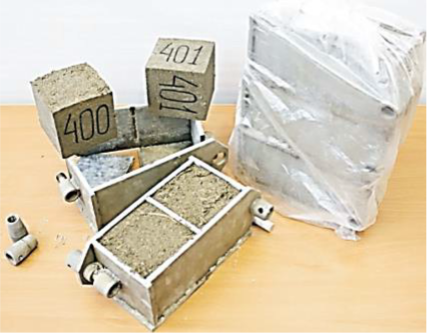
\includegraphics[width=0.6\textwidth]{media/chem/image2}
	\caption*{Рис.1 - Образец №1 на основе портландцемента}
\end{figure}

\begin{multicols}{2}
Образец № 1: органический наполнитель - СН 549-82, опилки древесные
массой 365 кг; вяжущее -- портландцемент М400 массой 317 кг; добавки --
известь гидратная 16 кг, жидкое стекло 43 кг, сульфат алюминия 20 кг;
армирование -- полипропиленовое фиброволокно длиной 18 мм, массой 1 кг;
влажность составляет 32-38\%, водоцементное отношение примерно 0,8 (вода
250 дм³).

Образец № 2: органический наполнитель -- СН 549-82, опилки древесные
массой 365 кг; вяжущее -- портландцемент М400 массой 317 кг; добавки --
известь гидратная 16 кг, жидкое стекло 43 кг, сульфат алюминия 20 кг;
армирование отсутствует; влажность составляет 32-38\%, водоцементное
отношение равно 1,0.

Образец № 3: органический наполнитель -- опилки древесные массой 350 кг;
вяжущее -- портландцемент М400 массой 300 кг, зола ТЭЦ 12; добавки --
известь гидратная 45 кг, жидкое стекло 45 кг, сульфат алюминия 15 кг;
армирование -- полипропиленовое фиброволокно длиной 18 мм, массой 1 кг;
влажность составляет 32-38\%, водоцементное отношение 1,1 (вода 330
дм³).

Образец № 4: органический наполнитель -- опилки древесные массой 350 кг;
вяжущее -- портландцемент М400 массой 300 кг, зола ТЭЦ 5; добавки --
известь гидратная 45 кг, жидкое стекло 45 кг, хлорид кальция 15 кг;
армирование отсутствует; влажность составляет 32-38\%, водоцементное
отношение 1,1 (вода 330 дм³).

Образец № 1. Форма заполнялась послойно, каждый слой уплотнен, визуально
смесь полусухая. Образец вынимали из формы через 24 часа. Исследования
проводили при температуре 20 0C. Длительность 28 дней (рисунок 1).

Изменение массы наблюдали в течении 28 суток, данные предоставлены на
графике зависимости массы от времени (рисунок 2). Масса образца
изменилась с 0,91 кг до 0,598 кг. Среднее значение плотности материала
образцов в возрасте 28 суток равно 595 кг/м\textsuperscript{3}.
\end{multicols}

\begin{figure}[H]
    \centering
    \begin{subfigure}[b]{0.4\textwidth}
        \centering
        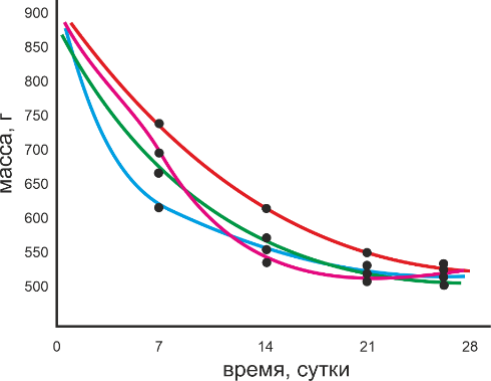
\includegraphics[width=\textwidth]{media/chem/image3}
        \caption*{Рис.2 - Зависимость изменения массы арболита от длительности эксперимента}
    \end{subfigure}
    ~
    \begin{subfigure}[b]{0.5\textwidth}
        \centering
        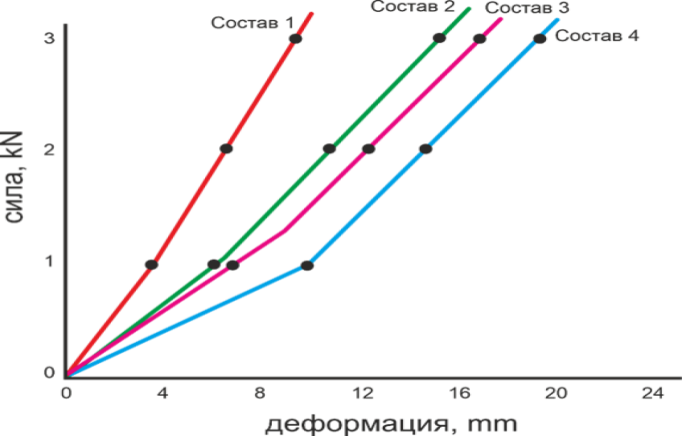
\includegraphics[width=\textwidth]{media/chem/image4}
        \caption*{Рис.3 - Зависимость сжатия образцов от укладки смеси}
    \end{subfigure}
\end{figure}

\begin{multicols}{2}
Образец был подвергнут сжатию вдоль и поперек слоям укладки цементного
теста. Образцы 1, 2, 3 разрушены, образец 4 показал прессование и
остаточные деформации.

Результаты испытаний для трех образцов приведены на графике зависимости
сила-деформация на рисунке 3. Зависимость прочности композитов от
направления укладки смеси при изготовлении важно для строительных работ.
Результаты исследований представлены на рисунке 3.

Образец №1. В качестве добавки был использован хлорид кальция, вместо
сульфата алюминия. В результате значительно увеличились прочность и
жесткость образцов.

Образец №2. Прочность образца ниже, чем №1. Жесткость уменьшилась.

Образец №3 При совместном использование извести и жидкого стекла
прочность образцов уменьшилась.

Образец №4 При совместном использование цемента и золы ТЭЦ. Добавки золы
ТЭЦ положительно влияют на свойства.

Основываясь на данные из литературных источников, были проведены
исследованию по использованию в качестве минеральной добавки порошка
талькохлора, который является отходом. Результаты испытаний показали,
что порошок талькохлорита могут заменить известь, и прочность образцов
увеличивается, тогда как применение смеси извести и порошка
талькохлорита снижает прочность и жесткость образцов. Увеличение
водоцементного отношения отрицательно сказывается на прочностных
характеристиках, хлорид кальция продает большую прочность арболиту, чем
сульфат алюминия. По ГОСТ Р 54854-2011 по критерию средней плотности
соответствует D600, это конструкционно теплоизоляционный материал. По
результатам исследований, класс прочности на сжатие соответствует марке
М10. Полученные данные соответствуют известным данным о закономерностях
изменения механических свойств древесно-цементных материалов, к которым
относится арболит {[}17-18{]}.

\emph{Технология изготовления арболита}

Ежегодно в Казахстане образуется более 15 млн. м\textsuperscript{3}
древесных отходов. Современные экологические требования и возможность
современных технологий ориентированы как на утилизацию этих отходов, так
и на использование их в составе различных современных материалов.
Применяемые композиционные материалы на основе отходов древесины имеют
разнообразное назначение во многих отраслях экономики страны, в том
числе для в древесно-цементных смесям для изготовления теплоизоляционных
и конструкционных строительных материалов. При этом материал должен
отвечать требованиям экологической чистоты в процессе изготовления,
эксплуатации и утилизации. Создание новых эффективных, экологически
чистых композиционных древесных материалов и разработка технологии их
получения, расширяет область использования древесных отходов
{[}19-20{]}.
\end{multicols}

\begin{figure}[H]
	\centering
	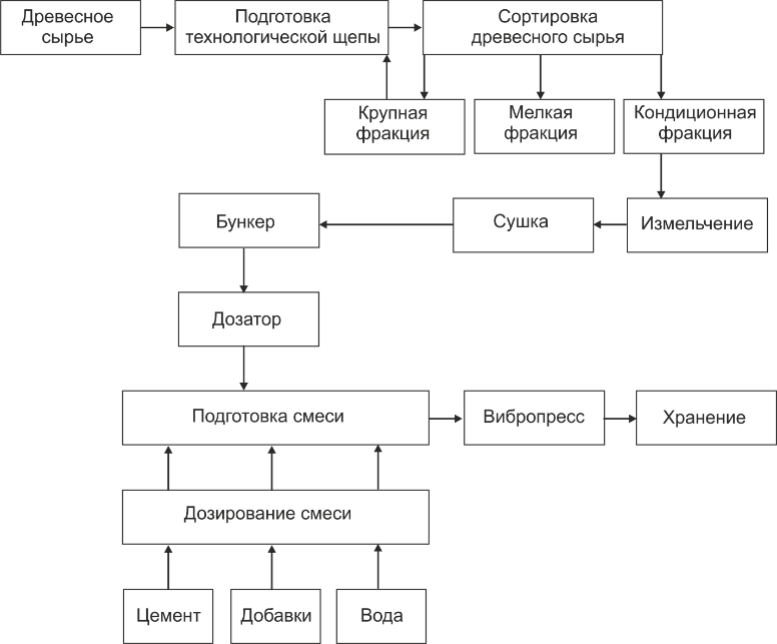
\includegraphics[width=0.8\textwidth]{media/chem/image5}
	\caption*{Рис.4 - Блок-схема технологического процесса арболитных блоков}
\end{figure}

\begin{multicols}{2}
Разработанная технология изготовления композиционного
древесно-цементного материала на основе древесных отходов содержит
небольшое количество основных технологических операций. Это
приготовление стружки, приготовление смеси для арболита и формирование
продукта в формы с вибропрессованием. Предварительно древесное сырье
выдерживается в помещении с плюсовой температурой более 2-х месяцев.
Блок-схема технологического процесса представлена на рисунке 4.

Для производства арболитных блоков, учитывая результы проведенных
иссследований по подбору компонентов смеси и проведенных испытаний
образцов, была выбрана рецептура для прочных и недорогих блоков. В
качестве минеральной добавки выбрали гидратную известь, хотя порошок
талькохлора показал лучшие результаты по прочности, данных по применению
пока недостаточно. Плотность готового влажного арболита должна быть в
пределах 900-980 кг/м\textsuperscript{3}; Плотность абсолютно сухого
арболита в пределах 620-750 кг/м3. Последовательность введения
компонентов в смеситель:

дробленку, водный раствор извести перемешивают, затем вводят раствор
сернокислого алюминия, цемент и остаток воды, смесь перемешивают 1,5-2
часа. Смесь содержит: портландцемент М 400 -- 25-30; известь гидратная
-- 30-435; сернокислый алюминий -- 10-20; древесная стружка -- до30;
вода -- 20-30.

Разработанная технология обладает простотой, экологической безопасностью
и универсальностью в части возможности изготовления арболита на основе
древесных отходов с широким спектром физико-механических свойств путем
варьирования компонентным составом с целью удовлетворения требований
условий эксплуатации готового изделия.

{\bfseries Выводы.} На основании представленных результатов по исследованию
рецептуры, технологии и свойств изделий из арболита, можно сделать вывод
о перспективности производства подобных древесно-цементных композитов,
лёгкими, прочными и с высокими тепло- и звукоизоляционными свойствами.

Проведены исследования компонентного состава смеси, влияния минеральных
добавок на адгезионные свойства и прочность готовой продукции.
Установлена эффективность применения золы ТЭЦ экибазтузскикого угля для
получения композитных строительных материалов. Исследовано влияние
влажности, крупности и качественных характеристик древесного наполнителя
на качество цементной смеси и прочностные характеристики изделий.

Анализируя полученные результаты, установлено, что по большинству
показателей, в частности: звукоизоляционным свойствам, легкому весу,
пористости, низкой теплопроводности, теплоемкости, огнеустойчивости,
неподверженности биоразложению, изделия из арболита соответствуют
требованиям, предъявляемым подобным строительным материалам.

Определена возможность получения готовых строительных блоков по
упрощенной технологии, с формированием изделий на вибростоле, что
позволяет использовать различные формы и производить изделия различных
размеров, использовать многокомпонентные, разные по характеристикам
смеси, дает возможности применения армирующих волокон и конструкций, что
увеличивает ассортимент продукции, без значительного дополнительного
оборудования.

В опытно-экспериментальном металлургическом производстве АО «ИМиО» было
запущено производство ФТП, на данное время производственная мощность
предприятия составляет 15 000 м\textsuperscript{2} теплоизолирующей
продукции в год.

Урбанизация предполагает рост строительства жилых зданий и промышленных
помещений, увеличивается спрос на недорогие, качественные и экологичные
строительные материалы. Возможность увеличения качества,
функциональности стройматериалов при сохранении невысокой стоимости за
счет использования вторичного сырья соответствующего качества,
предполагает актуальность дальнейшего проведения исследований технологий
и организации производства композитов.

\emph{{\bfseries Финансирование}. Данное исследование выполнено при
поддержке ТОО «URBAN GROUP» в рамках проекта DP21681444 «Организация
безотходного производства композиционных материалов из древесных
отходов».}
\end{multicols}

\begin{center}
{\bfseries References}
\end{center}

\begin{references}
1. Ребиндер П. А., Щукин Е. Д. Поверхностные явления в твердых телах в
процессах их деформации и разрушения //Успехи физических наук.-1972.-Т.
108(9). - С.3-42.

DOI
\href{https://doi.org/10.3367/UFNr.0108.197209a.0003}{10.3367/UFNr.0108.197209a.0003}

2. Новицкий А. Г., Ефремов М. В. «Особенности получения непрерывного
химически стойкого базальтового волокна» // Хімічна промисловість
України.2003. № 1. С.24-27.
\href{https://novitsky1.narod.ru/basalt5.htm}{https://novitsky1.narod.ru}

3. Толмачев С. Н., Беличенко Е. А., Холодный А. Г. Технологические,
механические и структурные характеристики цементных систем с углеродными
коллоидными частицами // Строительные материалы. -2010.-№.9. - С.96-100
\href{https://cyberleninka.ru/article/n/tehnologicheskie-mehanicheskie-i-strukturnye-harakteristiki-tsementnyh-sistem-s-uglerodnymi-kolloidnymi-chastitsami}{https://cyberleninka.ru}

4. Wang L. et al. Value-added recycling of construction waste wood into
noise and thermal insulating cement-bonded particleboards //Construction
and Building materials. -2016.-Vol.125. - P.316-325.
\href{https://doi.org/10.1016/j.conbuildmat.2016.08.053}{DOI
10.1016/j.conbuildmat.2016.08.053}

5. Moslemi, A.A., Y.T. Lim. Compatibility of southern hardwoods with
Portland cement // Forest Prod. J. - 1984. -- Vol.34(8).- P.22-26.

6. American Society for Testing and Materials. Heat of hydration of
hydraulic cement. ASTM // ASTM, West Conshohocken.2017. -- Р.186-191.
\href{https://ru.scribd.com/document/526400532/C186}{https://ru.scribd.com}

7. Sauvat, N., R. Sell, E. Mougel, A. Zoulalian. A study of ordinary
Portland cement hydration with wood by isothermal calorimetry //
Holzforschung. - 2005. - № 53(1). -- Р.104-108.
\href{https://doi.org/10.1515/HF.1999.016}{DOI 10.1515/HF.1999.016}

8. Лесовик В. С., Гридчина А. А. Монолитные бетоны на основе расширяющих
добавок и химических модификаторов //Строительные материалы.-2015.-№.8.
- С.81-83.

9. Сеничев В.П., Воропай Л.М., Осипов Ю.Р., Шлыков С. А. Влияние
фракционного состава древесного заполнителя на физико-механические
показатели арболита.//Вестник Череповецкого госудаоственного
университетаю-2015.- № 6.-С.47-50.

10. Новицкий А. Г., Ефремов М. В. «Аспекты применения базальтовой фибры
для армирования бетонов» // Будівельнi матеріали, вироби та санітарна
техніка.- 2010.-№ 36.-С.22-26.
\href{http://www.irbis-nbuv.gov.ua/cgi-bin/irbis_nbuv/cgiirbis_64.exe?I21DBN=LINK&P21DBN=UJRN&Z21ID=&S21REF=10&S21CNR=20&S21STN=1&S21FMT=ASP_meta&C21COM=S&2_S21P03=FILA=&2_S21STR=bmvs_2010_36_5}{}

11. Попов К.Н. Оценка качества строительных материалов / К.Н.Попов,
М.Б.Каддо, О.В. Кульков. - 2-е изд., перераб. и доп. -- М.: Высшая
школа, 2004.- 287 с. ISBN5-06-004283-9

12. Микульский В.Г., Куприянов В.Н., Сахаров Г.П. Строительные
материалы.- М.: Изд-во АСВ, 2000. -- 536 с. ISBN 5930930414.

13. Aigbomian E.P., Fan M. Development of Wood-Crete from Hardwood and
Softwood Sawdust // Open Construction and Building Technology
Journal.-2013.-Vol.7.-P.108--117.
DOI\\
\href{http://dx.doi.org/10.2174/1874836801307010108}{10.2174/1874836801307010108}

14. Филичкина М.В., Абрамов В.В., Самошин Д.С., Фролов Г.А. Особенности
опилок как наполнителя при производстве материалов из древесных отходов
// Лесотехнический журнал.-2013.-№ 2 (10).- С.26--30.

15. Лукутцова Н.П., Горностаева Е.Ю., Карпиков Е.Г. Древесно-цементные
композиции с

минеральными микро-наполнителями // Вестник БГТУ им. В.Г. Шухова.-
2011. -№ 3.-С.21-23

16. Цепаев, В. А.~О предельном уровне напряжения сжатия в кладке из
опилкобетона // Жилищное строительство. - 2008. -№ 9. - С.8-9.

17. Копарев В. С. Перспективы использования скопа в качестве сырья для
производства древесно-цементной композиции //Актуальные направления
научных исследований XXI века: теория и практика.- 2014.-Т.2(3), ч.2.-
С.92-95

18. Субботина Н.В., Саркисов Ю.С., Горленко Н.П., Чернов Е.Б. Влияние
состава и структуры жидкости затворения на свойства древесно-цементных
композиций // Вестник науки Сибири.- 2012.-Т.5 (6).- С.261--268.

19. Чемоданов А.Н., Горинов Ю.А., Сафин Р.Г. Композитный
теплоизоляционно-балластный материал на основе древесных отходов //
Безопасность жизнедеятельности.- 2015. - № 3. - С.63-67.

20. Андреев Г., Корженецкий А., Молчанова Л. Строительство Балхашской
ТЭС: современные технологии для устойчивого развития региона и снижения
уровня риска для здоровья населения // Энергетика. - 2014. - № 1(48). --
С.26-31.
\end{references}

\begin{authorinfo}
\emph{{\bfseries Information about authors}}

Ilmaliev Zh.B. - Senior Researcher, Senior Researcher, «URBAN GROUP» LLP
, Almaty, Kazakhstan, e-mail:
\href{mailto:jans2009@mail.ru}{};

Kurtibay K.A. - Master' s student, Research Associate of
«Scientific and Production Center of Ecological and Industrial
Biotechnology» LLP, Astana, Kazakhstan, e-mail:
\href{mailto:kurtibayqb@gmail.com}{};

Kappassuly A. - Master of Engineering and Technology, Research
Associate, «Scientific and Production Center of Ecological and
Industrial Biotechnology» LLP, Astana, Kazakhstan, e-mail:
\href{mailto:kappasuly@mail.ru}{}

Zhatkanbayev Ye.Ye. - Doctor of Technical Sciences, Associate Professor,
Kazakh University of Technology and Business named after K. Kulazhanov,
Astana, Kazakhstan, e-mail:
\href{mailto:erlan.ntp@mail.ru}{};

Ilmalieva G.B. - candidate of chemical sciences, researcher, «URBAN
GROUP» LLP Almaty, Kazakhstan, e-mail:
\href{mailto:g.ilmaliyeva@qazindustry.gov.kz}{};

Zhunussova E.B. - Candidate of Technical Sciences, Associate Professor,
Kazakh University of Technology and Business named after K.Kulazhanov,
Astana, Kazakhstan, е-mail:
\href{mailto:tahmina.66@mail.ru}{};

Zhumabekova A.K. - Kazakh University of Technology and Business,
Candidate of Chemical Sciences, Associate Professor, Astana, Kazakhstan,
е-mail:
\href{mailto:zhumabekova_ak@mail.ru}{}

\emph{{\bfseries Сведения об авторах}}

Ильмалиев Ж.Б. -старший научный сотрудник, ТОО «URBAN GROUP», Алматы,
Казахстан, e-mail:
\href{mailto:jans2009@mail.ru}{};
https://orcid.org/0000-0002-0979-0665

Куртибай Қ.А.- магистрант естественных наук, научный сотрудник ТОО
«Научно-производственный центр экологической и промышленной
биотехнологии», Астана, Казахстан, e-mail:
\href{mailto:kurtibayqb@gmail.com}{};
https://orcid.org/0000-0001-7822-0263

Қаппасұлы Ә. - магистр техники и технологии, научный сотрудник ТОО
«Научно-производственный центр экологической и промышленной
биотехнологии», Астана, Казахстан, e-mail:
\href{mailto:kappasuly@mail.ru}{};
https://orcid.org/0009-0000-6205-7721

Жатканбаев Е.Е.-д.т.н., ассоциированный профессор, Казахский университет
технологии и бизнеса имени К. Кулажанова, Астана, Казахстан, e-mail:

https://orcid.org/0000-0003-0656-239X

Ильмалиева Г.Б. -- к.х.н., научный сотрудник ТОО «URBAN GROUP», Алматы,
Казахстан,

e-mail:
\href{mailto:g.ilmaliyeva@qazindustry.gov.kz}{};
https://orcid.org/0009-0006-3649-0509

Жунусова Э.Б. - кандидат технических наук, ассоциированный профессор,
Казахский университет технологии и бизнеса им. К. Кулажанова, Астана,
Казахстан, e-mail:
\href{mailto:tahmina.66@mail.ru}{};
http://orcid.org/0000-0002-9844-6291

Жумабекова А.К. - кандидат химических наук, ассоциированный профессор,
Казахский университет технологии и бизнеса, г. Астана, Казахстан,
е-mail:
\href{mailto:zhumabekova_ak@mail.ru}{},
https://orcid.org/0000-0001-6743-8953.\
\end{authorinfo}
